\section{Statement of the Problem}
The study configuration is considered cylindrical. A scheme of the study geometry is given in Figure~\ref{figure:problem}:
\begin{figure}
	\centering
	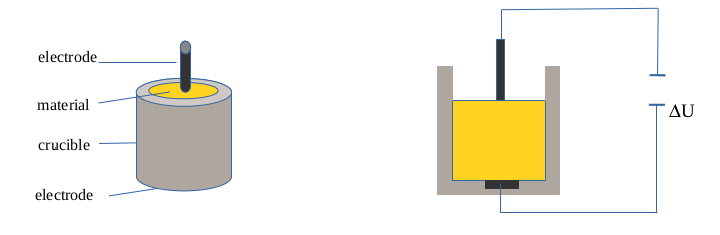
\includegraphics[height=4cm]{Images/problem.png}
	\caption{Problem Scheme}
	\label{figure:problem}
\end{figure}
The process is constituted by:
\begin{itemize}
	\item a cylindrical crucible;
	\item the elaborated material; the geometry of the study domain occupied by the material is cylindrical;
	\item 2 electrodes.
\end{itemize}

The electrodes are in graphite. An electrical potential difference is applied between the top electrode and the bottom electrode included in the crucible: $ \Delta U $. This electrical potential difference is \emph{continuous}. An electrical current pass through the material placed in the crucible. We suppose that the contact between the electrodes and elaborated material is perfect. \textbf{Joule effect heat the material}. The material of the crucible is an insulating material. The crucible is not model and will be replaced by an adapted boundary condition. Electrical problem has to be solved in the electrodes and in the elaborated material. The heat transfer has to be solved in the material only.

\section{Equations of the physical phenomenon and Boundary Conditions}
The objective of this part is to present the physical equations of the process in the steady state and boundary conditions. In this process two physical phenomena occur:
\begin{itemize}
	\item electrical phenomenon;
	\item thermal phenomenon.
\end{itemize}
\subsection{Presentation of the study domain}
Describe the study domain. Precise where each phenomenon is solved.
\begin{mdframed}
	The study domain is the one described in Figure~\ref{figure:problem}, right part. 
	\begin{itemize}
		\item We will solve the \textbf{thermal problem} only in the material only (yellow part), i.e.~where $ 0.1<r<0.3 $ and $ 0<h<0.3 $.
		\item We will solve the \textbf{electrical problem} in the electrodes and in the elaborated material, i.e.~for $ 0\geq r<0.3 $ and $ 0<h<0.3 $.  
	\end{itemize} 
\end{mdframed}
\subsection{Electrical problem}
Give the partial differential equation of the electrical problem.
Give the boundary conditions of the electrical problem.
Give the expression of the current density and of the Joule power density.
\begin{mdframed}
	The Electrical problem can be modeled employing the fact that $ E=-\nabla U $. We also now that the electrical flux is defined through $ \vec{J}\cdot \vec{E} $. Using the fact that the divergence of the Electrical flux is 0 we obtain that:
	\[ \nabla\cdot(-\sigma\nabla U)=0. \]
	We focus now on the boundary conditions: we know that around the crucible there's insulator material, then we'll have that $ \pd{U}{x}=0 $ on the boundary, i.e. $ \nabla U\cdot \vec{n}=0 $. We can also take into consideration that $ \Delta U $ is fixed and so we can write the final system as
	\[
	\begin{cases}
	\nabla\cdot(-\sigma\nabla U)=0, & 0<x<0.1,\,0.02<z<0.42\\
	\nabla U\cdot \vec{n}=0,& x\in \partial V\\
	U = \Delta U, & 0<x<0.02,\,z=0.4\\
	U=0, & 0<x<0.04,\,z=0.
	\end{cases}
	\]
\end{mdframed}

\subsection{Thermal problem}
\begin{itemize}
	\item Give the partial differential equation of the thermal problem.
	\item Give the boundary conditions of the thermal problem.
\end{itemize}
A medium through which electric current is conducted may involve the conversion of electrical or chemical energy into heat (or thermal energy), like in our case (i.e., Joule effect). In heat conduction analysis, such conversion processes are characterized as heat (or thermal energy) generation.
For example, the temperature of a resistance wire rises rapidly when electric current passes through it as a result of the electrical energy being converted to heat at a rate of $ I^2R $, where $ I $ is the current and $ R $ is the electrical resistance of the wire. 
Note  that  heat  generation  is  a  volumetric  phenomenon. That  is, it  occurs throughout the body of a medium. Therefore, the rate of heat generation in a medium is denoted per unit volume. The rate of heat generation in a medium may vary with time as well as position within the medium. When the variation of heat generation with position
is known, the total rate of heat generation in a medium of volume $ V $ can be determined from
\[Q = \dot{q}=\int_V q_{gen}\diff V. \]
In  our case, where there's no time dependence on the process of heat  generation,  as  in  the  case  of  electric resistance heating throughout a homogeneous material, the relation reduces to 
\[Q = \int_{V}q\diff V. \]

The Fourier Law tells us that:
\begin{equation}
\label{eq:Fourier}
q=-k\nabla T
\end{equation}
where
\begin{description}
	\item[$ q$] local heat flux density,
	\item[$ k $] material's conductivity,
	\item[$ \nabla T $] is the temperature gradient. 
\end{description}

Using Fourier Law \eqref{eq:Fourier} and plugging it into the above equation we obtain
\begin{equation}
\nabla\cdot(-k\nabla T)=Q.
\end{equation}
The final system of equation will be
\begin{equation}
\label{problem:heat}
\begin{cases}
	\nabla\cdot(-k\nabla T)=Q, \\
	-\kappa\nabla T\cdot \vec{n}=h(T-T_r), &\text{on the upper surface},\\
	-\kappa\nabla T\cdot \vec{n}=0, &\text{on the non free surfaces}.
\end{cases}
\end{equation}


	
\section{Principle of the Modeling}
In this project, in a first step, each equation will be developed and test. In a second step, the model with the
two coupling equations will be developed and test. For numerical modeling the finite element method is
used. In this project, describe the steps of the calculation and the variables used. Take time to define how you
will present your numerical results.
